\section{Subgroup analysis}
\subsection{Countries and language regions}

\begin{figure}[htbp]
    \centering
    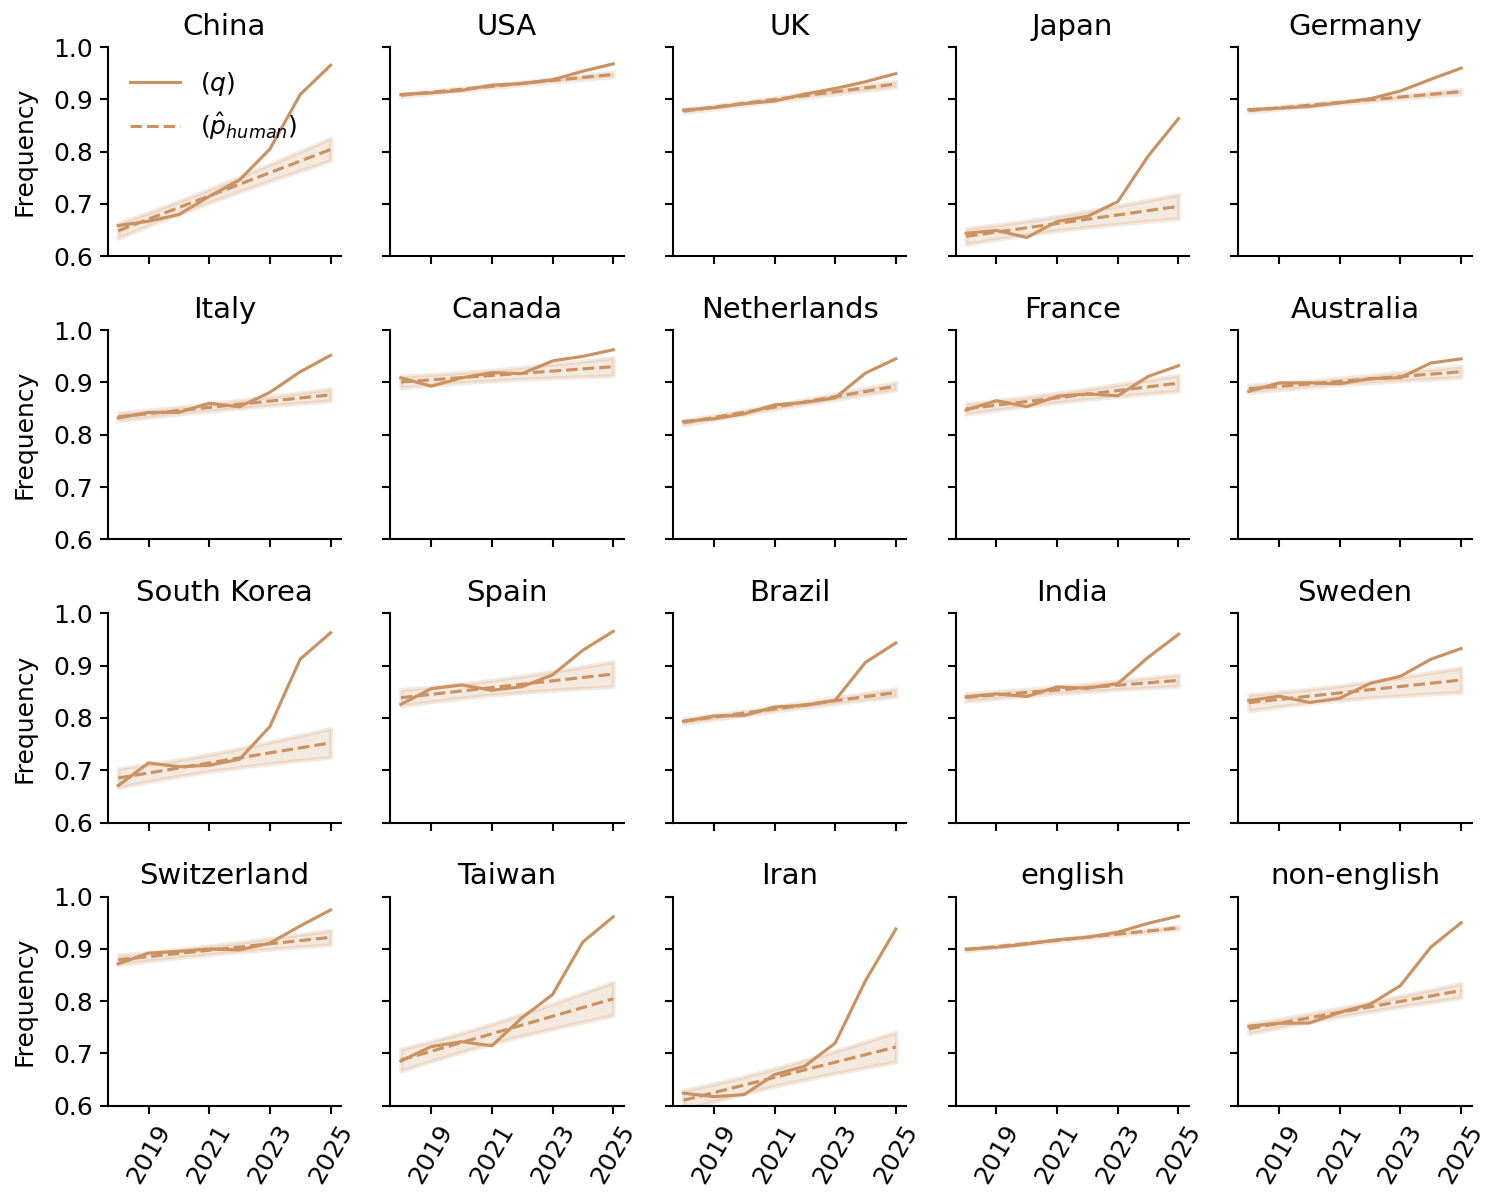
\includegraphics[width=\linewidth]{../results/plots/baseline_2026-01-23/research-article_aimrd_f/countries_individual_freqs_subsubopt.png}
    \caption{}
    \label{fig:countries_freqs}
\end{figure}

\subsection{Academic Discipline}\label{ap:disciplines}

\begin{figure}[htbp]
    \centering
    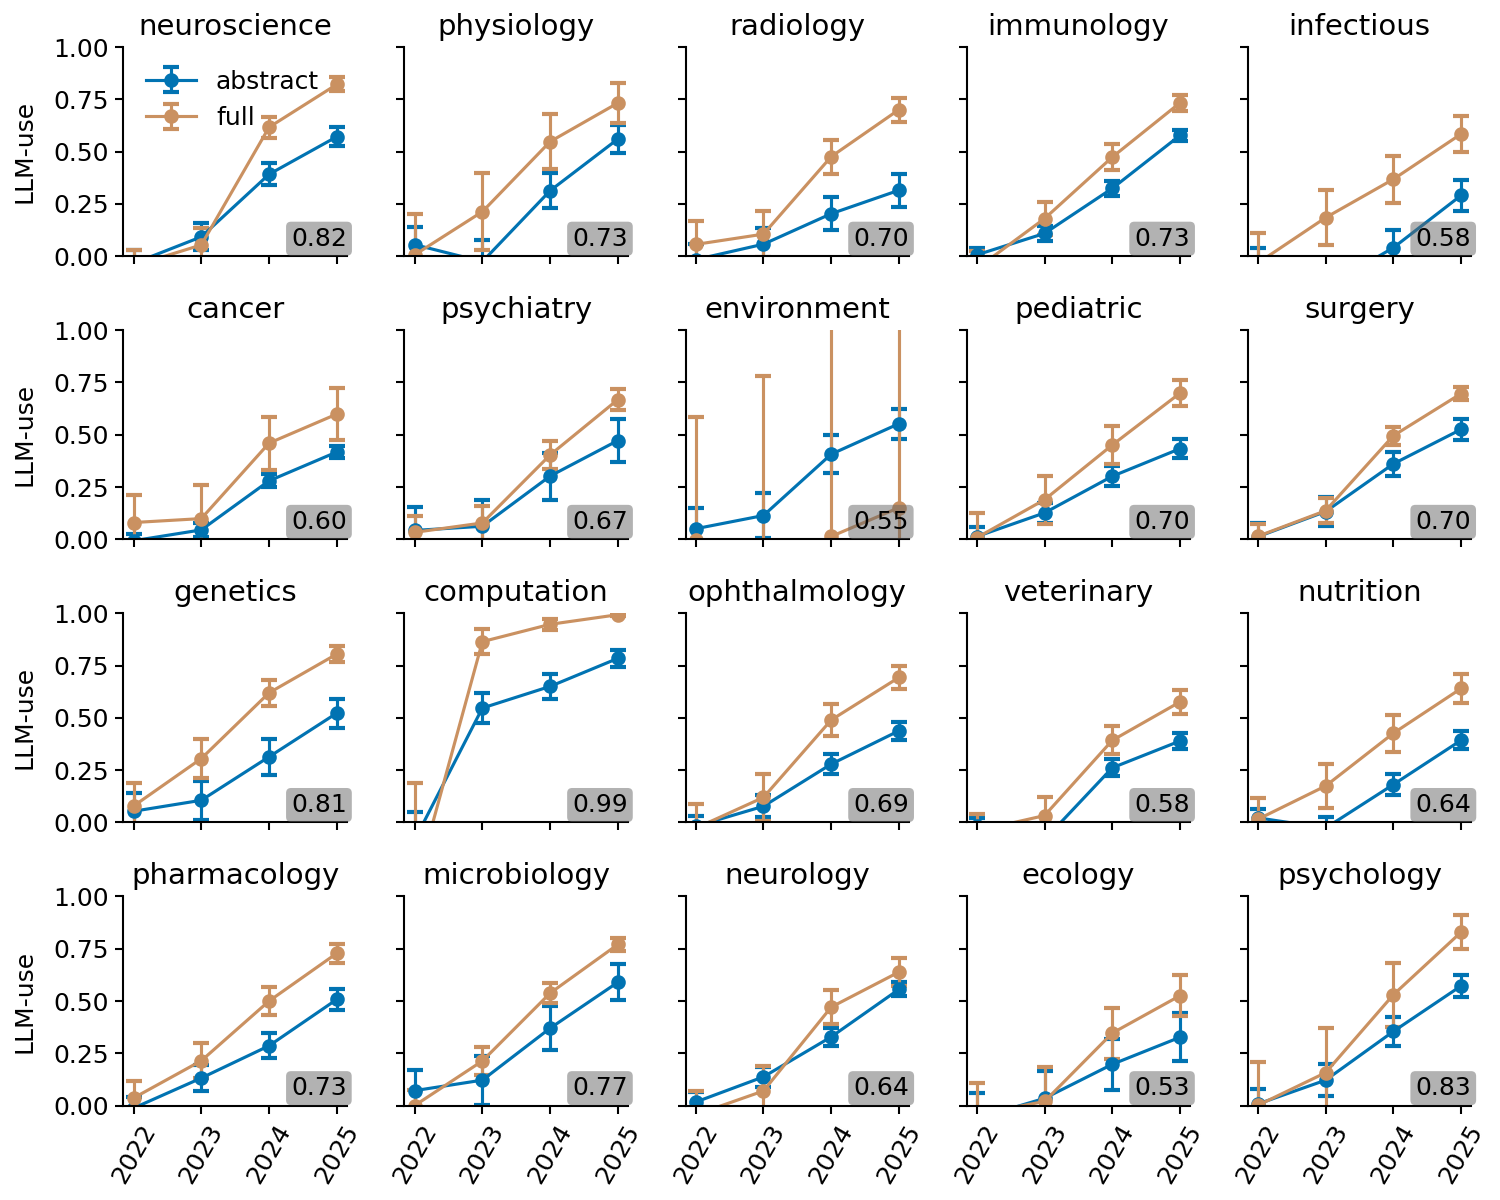
\includegraphics[width=\linewidth]{../results/plots/baseline_2026-01-23/research-article_aimrd_f/disciplines_individual.png}
    \caption{LLM-use estimates for different academic disciplines contributing to PMC for the abstract and main body of the paper. The highest estimate in each panel is marked in a gray box.}
    \label{fig:disciplines_ind}
\end{figure}

\begin{figure}[htbp]
    \centering
    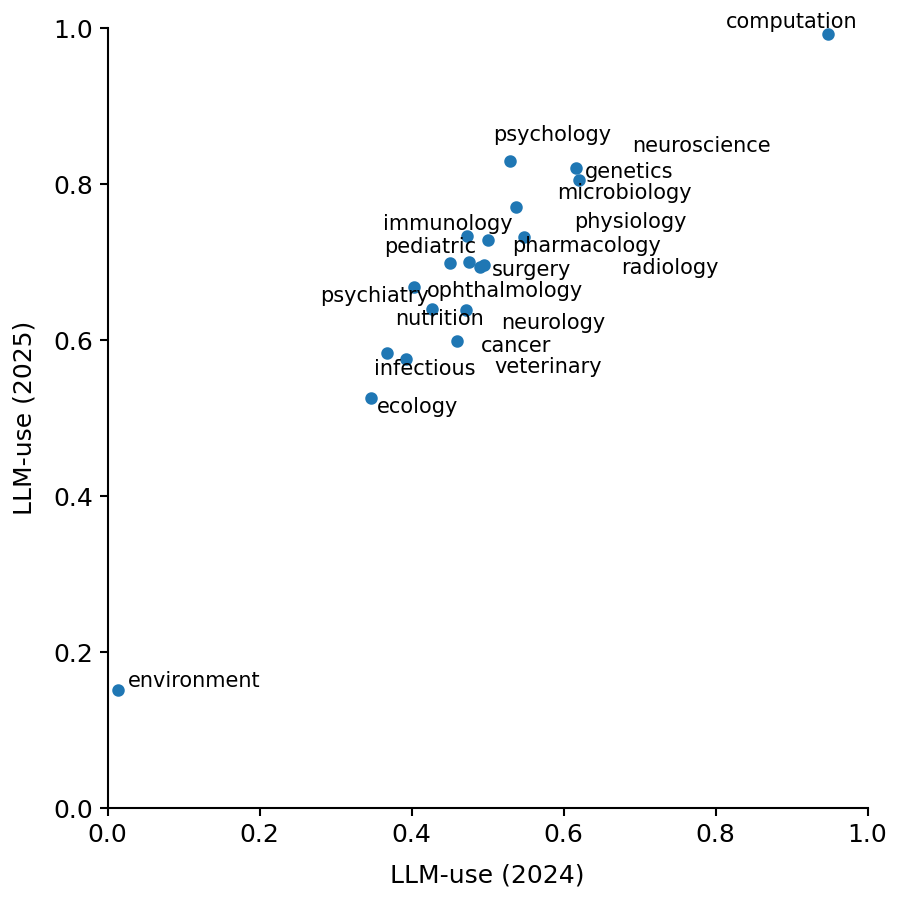
\includegraphics[width=\linewidth]{../results/plots/baseline_2026-01-23/research-article_aimrd_f/disciplines_2024v2025.png}
    \caption{LLM-use estimates of 2024 (x-axis) and 2025 (y-axis) for different academic disciplines. Because the number of papers in each category is very small, some estimates have very high uncertainty.}
    \label{fig:disciplines_all}
    %comment: this should be a different color than countries
\end{figure}